\begin{sectionbox}{La electricidad de nuestro cuerpo}
    \begin{minipage}{0.35\textwidth}
        La noche tormentosa del 16 de abril de 1786, en Bolonia, ciudad de Italia, el médico y físico
        Luigi Galvani (1737-1798) hizo pasar una descarga eléctrica proveniente de un rayo a través de las ancas de una rana que, casi
        de manera instantánea, comenzaron a moverse y a contraerse
        de manera violenta, como cuando le pertenecían a la rana.
        Sin embargo, lo más impresionante lo descubriría poco después al poner en contacto los nervios y músculos de las piernas
        de la rana con un arco compuesto por dos metales (cobre y zinc),
        y observar que éstas también se contraían. ¿Por qué las patas de la rana se movían si aparentemente no
        habían recibido una descarga eléctrica? Porque el sistema compuesto por los dos metales y las ancas actúan como una
        pila.
    \end{minipage}\hfill
    \begin{minipage}{0.6\textwidth}
        \begin{figure}[H]
            \centering
            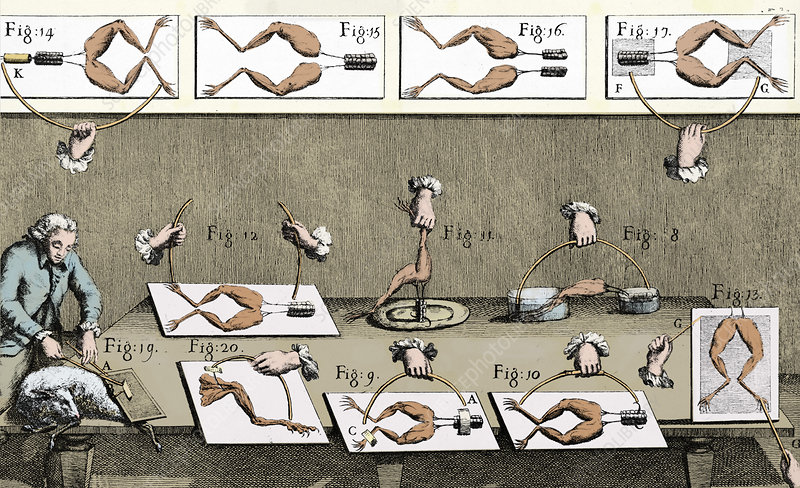
\includegraphics[width=0.95\linewidth]{../images/galvani01}
            \caption{Ilustración de 1792 sobre los experimentos de Galvani con ranas.}
            \label{fig:galvani01}
        \end{figure}
    \end{minipage}

    Las ancas conducen la corriente que se genera en esa pila y activan los
    movimientos de la rana. Galvani supuso que las patas de la rana poseían electricidad
    (a la que después llamó \comillas{electricidad animal}) y que esa era
    la causante de ese fenómeno. ¿Piensas que tenía razón, es
    decir, que los organismos poseen electricidad? ¿Esto explicaría las reacciones que observó en las piernas de la rana?
    En muchas de las funciones de un organismo interviene la electricidad. En condiciones normales, el organismo es capaz de generar las corrientes necesarias
    para cumplir sus funciones de forma autónoma, es decir, sin pilas ni descargas de
    rayos. En ese sentido, se puede decir que sí poseen electricidad propia. Pero en
    el experimento de Galvani, la rana está muerta y es la corriente externa la que
    produce las reacciones observadas.

    Imagina que mientras realizas esta guía escuchas el inoportuno sonido de la olla exprés
    que te encargaron retirar del fuego. Después de unos segundos, al levantarte de
    prisa, y sin querer, te golpeas un dedo del pie con la pata de una silla. Casi de inmediato retiras el pie y lanzas un grito de dolor, pero ¿cómo te diste cuenta de lo
    sucedido?, ¿cuánto tiempo tardaste en gritar?, ¿cómo recibió tu sistema nervioso
    tan rápido el mensaje de que te golpeaste?
    En tu curso de Ciencias y tecnología 1 estudiaste que el sistema nervioso se encarga de interpretar y procesar la información que recibimos del exterior y del
    interior de nuestro cuerpo (mediante los órganos de los sentidos), y que está compuesto por millones de neuronas que se enlazan entre sí y actúan en concierto,
    como los músicos de una orquesta, para que podamos pensar, sentir o movernos.
    Cuando recibimos un estímulo (percibimos un olor, un aumento de temperatura o
    recibimos un golpe en un dedo del pie) los órganos de los sentidos le informan al sistema nervioso a través de las neuronas; entonces el cerebro o la médula espinal emite
    una respuesta (¡aparta inmediatamente el dedo!), pero ¿cómo se comunican entre sí
    las neuronas?

    \begin{figure}[H]
        \centering
        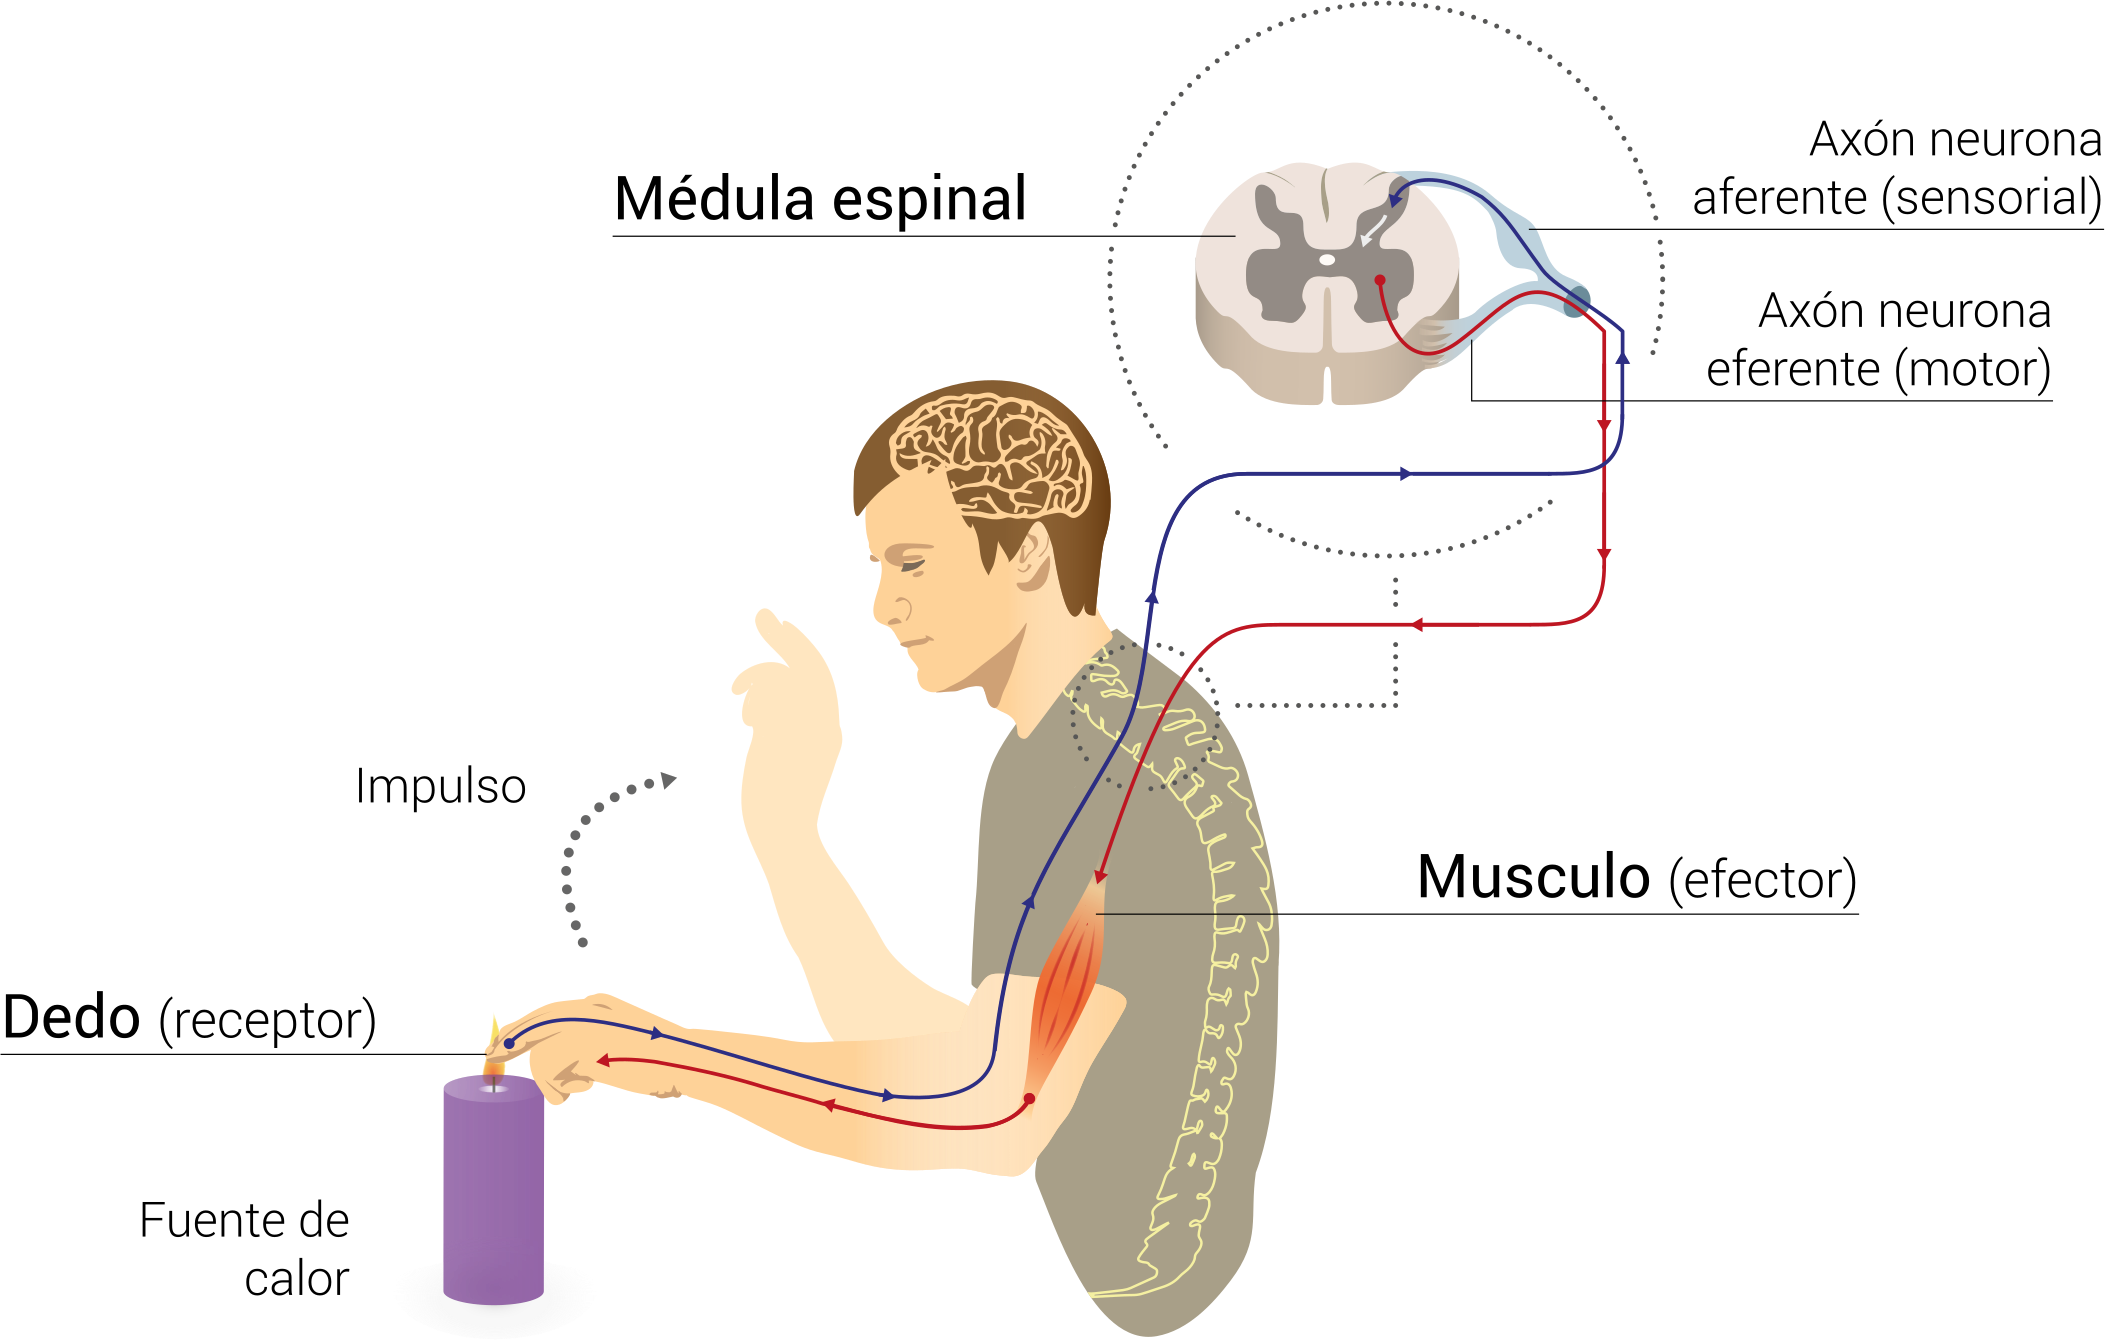
\includegraphics[width=0.8\linewidth]{../images/arcoreflejo}
        \caption{Un arco reflejo es el movimiento repentino que un individuo realiza de manera involuntaria ante un estímulo externo.}
        \label{fig:arcoreflejo}
    \end{figure}
    
\end{sectionbox}